\newcommand{\ClassPath}{../../VIU_TFM_LaTeX_template}
\documentclass{\ClassPath/viu-tfm-template}
\usepackage{multicol}

\definecolor{maincolor}{HTML}{f25416}

%--------------------------------------------------------------------------
% Definiciones necesarias Modifica con tus datos
%--------------------------------------------------------------------------
\def\nombre{Gómez Olivencia, Rubén}
\def\dni{78910013-A}
\def\titulo{Juego del solitario creado con \linebreak\linebreak HTML, CSS y Javascript}
\def\titulacion{Máster Universitario en Desarrollo de Aplicaciones y Servicios Web}
\def\curso{2022-2023}

%Los siguientes son opcionales: si no se ponen, la portada cambia un poco. Ideal para escribir artículos/trabajos cortos
\def\dirige{}
\def\convocatoria{}
\def\asignatura{Desarrollo de aplicaciones web II: lado del cliente (front-end) y multimedia}


% importar fichero de Bibliografía
%\addbibresource{Actividad_1.bib}

\begin{document}
    \graphicspath{{../../VIU_TFM_LaTeX_template/}}

    \coverpage

    \tableofcontents

\chapter{Introducción}

A lo largo de este documento se va a explicar las decisiones tomadas, tanto en el ámbito de programación como de diseño, a la hora de programar un juego basado en el popular juego de cartas “el solitario”.

Para la realización de este juego se ha hecho uso del lenguaje de marcado de hipertexto \textbf{HTML}, junto con el sistema de hojas de estilo en casacada \textbf{CSS} y el lenguaje de programación \textbf{Javascript}.


\chapter{Arquitectura cliente-servidor}
A la hora de realizar una aplicación web, o como en este caso un juego, tenemos que tener en cuenta cómo funciona la arquitectura que hace posible que podamos interactuar con ello.

Cuando navegamos por internet se hace uso de la conocida como arquitectura \textbf{Cliente - Servidor}, en la que podemos diferenciar, como su nombre indica, dos apartados:

\begin{itemize}
    \item \textbf{Servidor}: Un servidor es un ordenador potente que recibe peticiones, las procesa y devuelve una respuesta dependiendo de la petición recibida. En el caso de una aplicación web, el servidor contará con un servicio que recibirá peticiones \textbf{HTTP} y responderá con respuestas en código HTML, imágenes, ficheros ... Entre los servidores web más conocidos están: \href{https://httpd.apache.org/}{Apache HTTP Server}, \href{https://nginx.org/}{Nginx}, \href{https://www.iis.net/}{IIS}, ...

    \item \textbf{Cliente}: A la hora de interactuar con una aplicación web el cliente es quien va a realizar las peticiones al servidor. Normalmente el cliente es un navegador web utilizado por un usuario. Entre los navegadores web más conocidos están: \href{https://www.mozilla.org/es-ES/firefox/}{Firefox}, \href{https://www.google.com/chrome/}{Chrome}, \href{https://www.microsoft.com/es-es/edge}{Edge}, ...
\end{itemize}

A la hora de interactuar, un usuario hará uso del cliente (navegador web), con el que interactuará para realizar, normalmente, peticiones al servidor en busca de información. A continuación se puede ver un dibujo de cómo funciona la interacción descrita:


\begin{center}
    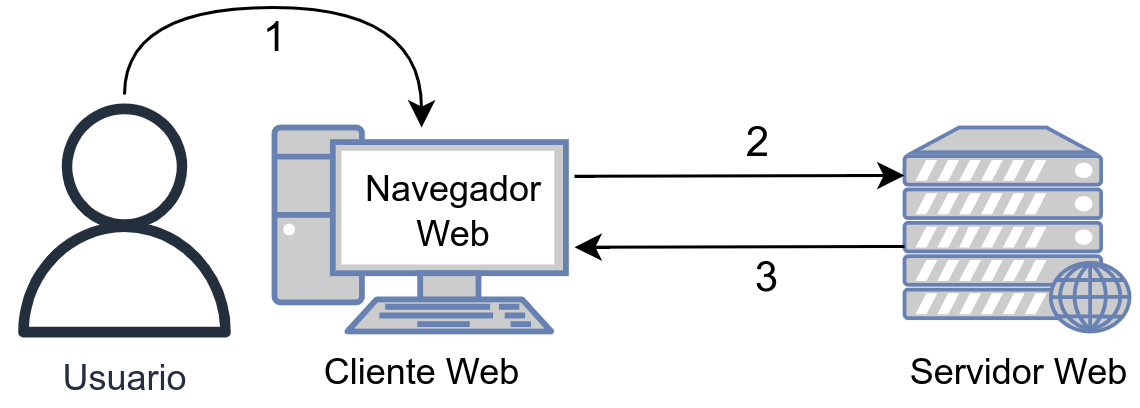
\includegraphics[width=0.6\linewidth]{img/cliente_servidor.png}
\end{center}

Tal como se puede ver en la imagen, los pasos que se realizan son:

\begin{enumerate}
    \item \textbf{Usuario interactúa con navegador web}. Tal como hemos dicho, un navegador web es el cliente de nuestra arquitectura, que es utilizado por el usuario. Cuando un usuario accede a una web, hace click en un enlace, realiza una búsqueda Google está comenzando el proceso del siguiente paso.

    \item \textbf{Realizar petición}. El navegador detecta lo que el usuario quiere realizar, y en ese momento lanza una petición (o varias) pidiendo al servidor web lo solicitado (una nueva web, una búsqueda, ...).

    \item \textbf{Devolver respuesta}: El servidor web recibe la petición, la procesa, y devuelve el resultado al cliente (navegador web) que la procesará y mostrará por pantalla.
\end{enumerate}

\section{Backend vs. Frontend}
En la arquitectura mostrada previamente, a la hora de diseñar el software, entran en juego también dos partes, que se encargarán por separado de procesar la entrada y realizar una salida:

\begin{itemize}
    \item El \textbf{Back end} es el software que se ejecuta en la parte de \textbf{servidor}, que recibe las peticiones del cliente, las procesa (gestión de autenticación, acceedr a base de datos, realizar cálculos, obtener información...) y que posteriormente el servidor devolverá.

    En este apartado de \textbf{backend} se hace uso de lenguajes de programación como \href{https://www.php.net/}{php} (junto con frameworks), frameworks como \href{https://rubyonrails.org/}{Ruby on Rails} o \href{https://www.java.com/es/}{Java}, por poner sólo unos pocos.

    \item El \textbf{Front end} es la parte que se ejecuta en la parte \textbf{cliente} (navegador web) de la arquitectura anterior. Mostrará la información atendiendo al diseño recibido, teniendo en cuenta la información HTML y las hojas de estilos CSS.

    También existe la posibilidad de ejecutar código que alterará, o que nos permitirá interactuar con la web. Este código está escrito en lenguaje \textbf{javascript} y que se ejecuta enteramente en el lado cliente (navegador web).
\end{itemize}

El juego realizado, que se va a detallar a continuación, ha sido realizado para que pueda ser ejecutado enteramente en la parte \textbf{frontend}. Esto hace que no sea necesario un servidor con el que interactuar, y por tanto sólo el navegador web ejecutará todas las funciones necesarias para poder jugar.


\chapter{Normas del juego}

Aunque el juego del solitario es conocido, a continuación se va a detallar brevemente las normas del juego, ya que es importante para entender el desarrollo realizado.

Las reglas del juego son las siguientes:

\vspace{-1em}
\begin{itemize}
    \item La baraja de cartas consta de:
    \begin{itemize}
        \item 4 palos nombrados como “viu”,”cuadrados”, “hexágonos” y “círculos”. Los dos primeros tienen color naranja y los dos últimos color gris.
        \item Cada palo tiene 12 cartas numeradas del 1 al 12.
    \end{itemize}
    \item La mesa de juego contará con seis tapetes (donde se colocarán los mazos de cartas).
    \item Los tapetes tienen las siguientes funciones:
    \begin{itemize}
        \item \textbf{Tapete inicial}: donde se sitúa el mazo completo ya barajado al inicio de la partida. Este tapete nunca podrá recibir cartas mientras haya cartas en él.
        \item \textbf{4 tapetes receptores}: donde se sitúan las cartas en orden decreciente (empezando siempre por una carta con el número 12) y alternando los colores. No se puede saltar ningún número y nunca podrán ir dos cartas del mismo color seguidas.
        \item \textbf{Tapete sobrantes/descartes}: donde se pondrán las cartas de manera temporal desde el tapete inicial ya que no es posible ponerlas sobre ningún tapete receptor.

        Es posible que si nos equivocamos podamos mover una carta de este tapete a uno receptor
    \end{itemize}

    \item Cuando no queden cartas en el tapete inicial, se cogerán las cartas del  tapete sobrantes, se barajarán y se pondrán sobre el tapete inicial.

    \item El juego termina cuando no haya ninguna carta sobre el tapete inicial ni el sobrantes.
\end{itemize}
\vspace{-1em}

La mesa de juego tiene la siguiente forma, donde se pueden ver los distintos tapetes, en la fila superior el inicial (más grande) y el sobrantes, y abajo los cuatro de recepción:
\begin{center}
    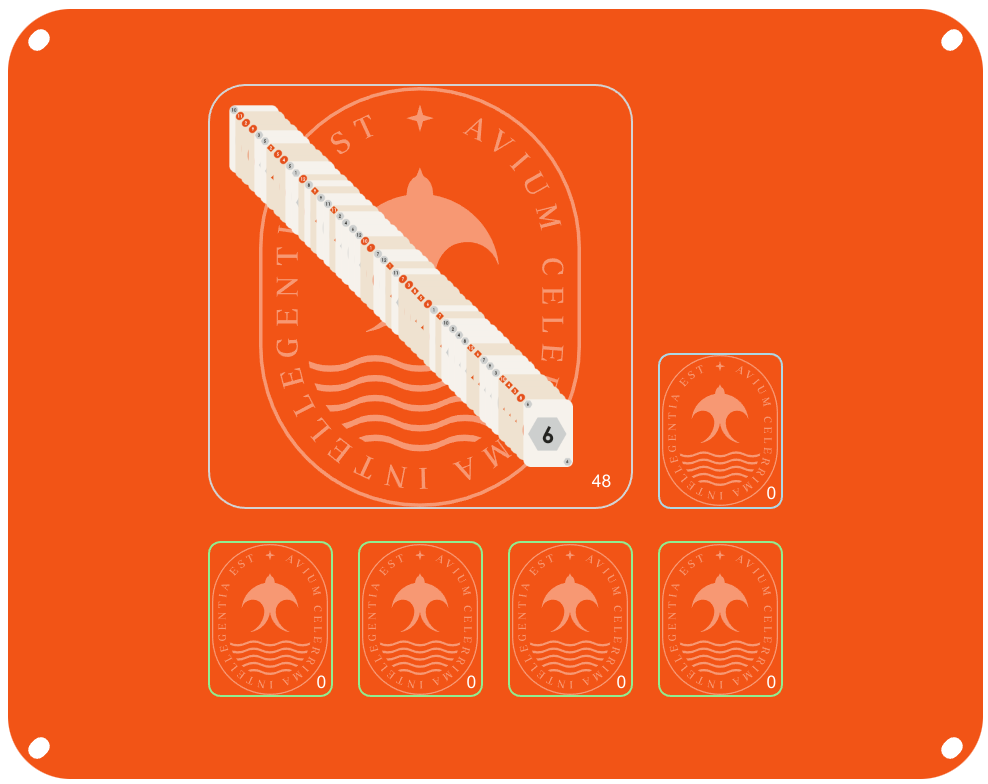
\includegraphics[width=0.7\linewidth]{img/mesa.png}
\end{center}


\chapter{Desarrollo realizado}

Teniendo en cuenta las reglas previas, se ha tenido que realizar el desarrollo acorde a las mismas para poder jugar. En este apartado no se va a detallar el aspecto visual del mismo, y nos vamos a centrar en la parte programada en \textbf{javascript}.

A la hora de realizar el desarrollo existen distintos aspectos y etapas que tiene el juego. A continuación se exponen y serán detallados más adelante:

\begin{itemize}
    \item Variables globales
    \item Comienzo del juego
    \begin{itemize}
        \item Barajar y cargar el tapete inicial
        \item Control del tiempo y contadores
    \end{itemize}
    \item Mover carta entre tapetes
    \item Fin del juego
\end{itemize}
\vspace{-1em}


\section{Variables globales}
A la hora de realizar el juego se han creado distintas variables globales que pueden ser accedidas desde cualquier parte del juego. Esto facilita el realizar cambios en los valores de las mismas.

Sin entrar en las variables de los palos y los números, existen tres variables globales principales que son las siguientes:

\vspace{-1em}
\begin{itemize}
    \item \textbf{Tapetes}: Los tapetes existentes en el juego.
    \item \textbf{Mazos}: Los mazos que habrá durante el juego, cada uno encima de un tapete distinto.
    \item \textbf{Contadores}: Los contadores que controlan cuántas cartas hay en cada tapete.
\end{itemize}
\vspace{-1em}

Cada una de estas tres variables son un array de seis posiciones, siguiendo el orden:

\vspace{-1em}
\begin{itemize}
    \item \textbf{Inicial}: Tiene que ver con el tapete/mazo inicial. Posición “0” del array.
    \item \textbf{Tapetes receptores}: Hay cuatro tapetes receptores, y por tanto cuatro posiciones en el array para cada uno de ellos (1..4).
    \item \textbf{Sobrante}: La última posición (5) es para el tapete sobrante, su mazo y el contador del mismo.
\end{itemize}
\vspace{-1em}

\section{Comienzo del juego}
Tal como se ha podido ver previamente, el comienzo del juego se ha diferenciado en dos apartados, que se realizan de manera consecutiva.

Para que comience el juego, primero debemos hacer click sobre el botón situado en la parte inferior con el aspecto:

\vspace{-1.6em}
\begin{center}
    
\includegraphics[width=0.2\linewidth]{img/boton.png}
\end{center}
\vspace{-1em}

\subsection{Barajar y cargar el tapete inicial}
Este apartado es el principal del juego, ya que se encarga de crear el mazo inicial  juntando las cartas de cada uno de los palos de la baraja.

Para ello se recorren los palos y las cartas y se añaden al array de mazos (posición “0”, de inicial). Se crean objetos imágenes, indicando cuál es el origen de la imagen a utilizar, indicamos que los objetos se pueden mover (“\textit{draggable}”) y añadimos ciertos atributos que después necesitaremos para aceptar o denegar el movimiento entre tapetes.

Este mazo inicial se baraja en la función \textbf{barajar}, que recibe el mazo como parámetro, que también se utilizará al pasar las cartas del tapete sobrantes al inicial.

Y por último, se colocan las cartas sobre el tapete inicial a través de la función \textbf{cargar\_tapete\_inicial} haciendo un efecto en cascada diagonal.


\subsection{Control del tiempo y contadores}
Este apartado no es estrictamente necesario en el juego, pero da valor a la hora de que sea más ameno si queremos tratar de batir nuestro propio récord, ya sea de tardar menos o realizar el menor número de movimientos posibles.

El juego cuenta con un control de tiempo, que es un \textit{timer} que se llama cada segundo, realizando un incremento de tiempo para posteriormente ser visualizado en el formato “HH:MM:SS” (donde “HH” son horas, “MM” minutos y “SS” segundos).

En lo que se refiere a los contadores, existe un contador para cada tapete, situado en su esquina inferior derecha, para saber de esta manera cuántas cartas tiene el mazo que está sobre él.

Y por último, existe el contador de movimientos, que se incrementa cada vez que movemos una carta sobre cada uno de los tapetes.

Tanto el tiempo como el contador de movimientos se puede ver en la parte superior de la página, encima de la mesa de juego:

\vspace{-1em}
\begin{center}
    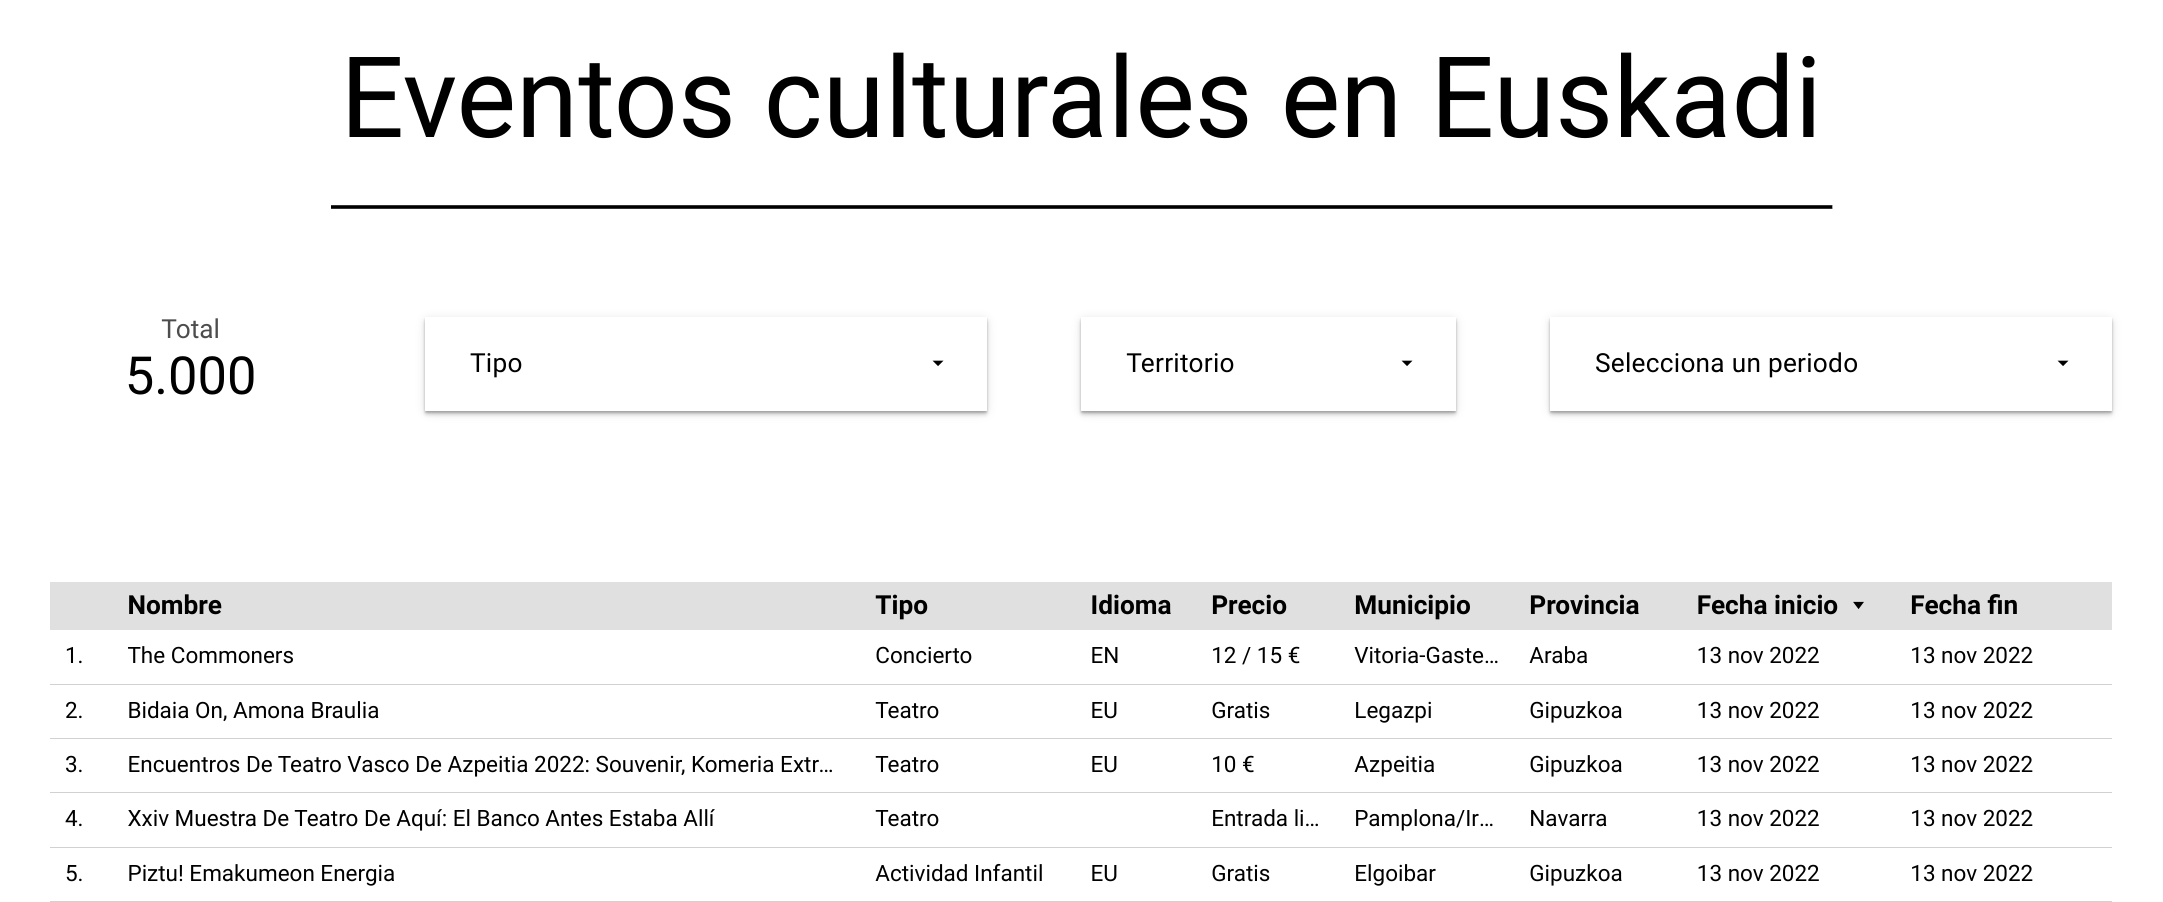
\includegraphics[frame,width=0.8\linewidth]{img/cabecera.png}
\end{center}
\vspace{-1em}

Tras esto, el botón que daba comienzo al juego se ha cambiado de color y ahora pone “Reiniciar”, lo que reiniciará el juego, limpiando tapetes, contadores, volviendo a barajar y situando las cartas de nuevo en el tapete inicial.

\vspace{-1.6em}
\begin{center}
    
\includegraphics[width=0.2\linewidth]{img/reiniciar.png}
\end{center}
\vspace{-1em}


\subsection{Mover carta entre tapetes}



\chapter{Aspecto visual}


\chapter{Conclusiones}


%\printbibliography[title={Referencias bibliográficas},heading=bibintoc]

\end{document}
